\section{Evaluation}

\begin{definition}[Approximation of the asymptotic complexity]
  Let $\BoundSet(\VSet)$ be a set of bounds over the variables $\VSet$.
  Let $\landau$ be the landau symbol for asymptotic complexity.
  Then, $\complexity$ is a function which assigns each bound an overapproximation of its asymptotic complexity.
  \[ \complexity(\infty) = \landau(\infty) \text{ for } \infty \in \BoundSet(\VSet) \]
  \[ \complexity(k) = \landau(1) \text{ for all } k \in \mathbb{N} \subset \BoundSet(\VSet) \] 
  \[ \complexity(v) = \landau(n) \text{ for all } v \in \VSet \subset \BoundSet(\VSet) \] 
  \[ \complexity(-b) = \complexity(b) \text{ for all } b \in \BoundSet(\VSet) \] 
  \[ \complexity(b_1 + b_2) = \landau(\complexity(b_1) + \complexity(b_2)) \text{ for all } b_1, b_2 \in \BoundSet(\VSet) \] 
  \[ \complexity(b_1 \cdot b_2) = \landau(\complexity(b_1) \cdot \complexity(b_2)) \text{ for all } b_1, b_2 \in \BoundSet(\VSet) \] 
  \[ \complexity(\max(b_1, b_2)) = \landau(\max(\complexity(b_1), \complexity(b_2))) \text{ for all } b_1, b_2 \in \BoundSet(\VSet) \]
  \[ \complexity(k^b) = k^{\complexity(b)} \text{ for all } k \in \mathbb{N} \subset \BoundSet(\VSet), b \in \BoundSet(\VSet) \]  
\end{definition}

For the parallel execution of the examples, we used the GNU tool 'parallel' \cite{gnuparallel}.

\begin{center}
  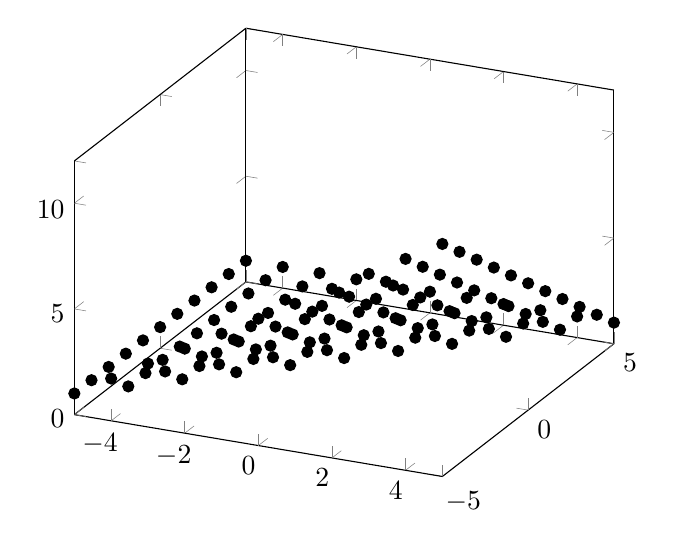
\begin{tikzpicture}
    \begin{axis}
      \addplot3 [
        unbounded coords=jump,
        mesh,
        shader=interp,
        samples at={-5,...,5},
        samples y={11},
        only marks,
      ] {1+max(x-y,0)};
    \end{axis}
  \end{tikzpicture}
  \hfil
  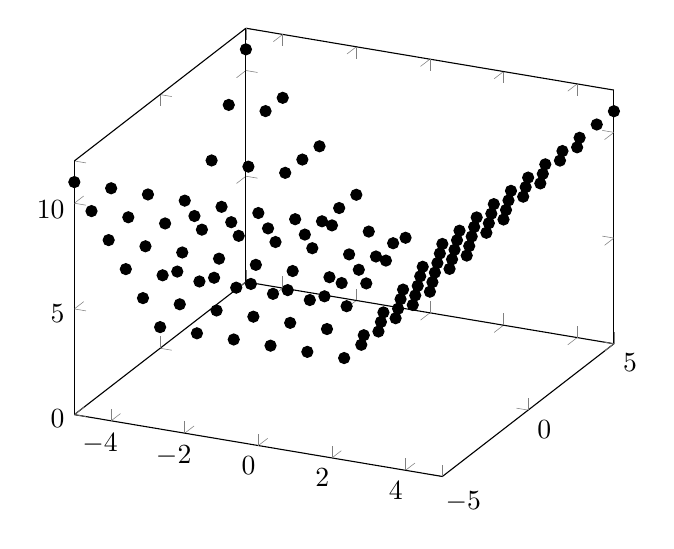
\begin{tikzpicture}
    \begin{axis}
      \addplot3 [
        unbounded coords=jump,
        mesh,
        shader=interp,
        samples at={-5,...,5},
        samples y={11},
        only marks,
      ] {1+abs(max(x,-y))+abs(max(x,-y))};
    \end{axis}
  \end{tikzpicture}
\end{center}
